% !TeX spellcheck = de_DE
\documentclass{alex_hü}

\name{Alexander Helbok}
\course{PS Physik}
\hwnumber{8}

\usetikzlibrary{arrows,calc, shapes.geometric, decorations.pathmorphing, matrix}
\tikzset{snake arrow/.style=
	{-Latex,
		decorate,
		decoration={snake,amplitude=.4mm,segment length=2mm,post length=1mm}},
}

\begin{document}
\renewcommand{\labelenumi}{\alph{enumi})}


\begin{mybox}{Reichweite von Alpha-Strahlung}
	\centering \begin{tabular}{c|c c c c c c c c c c c}
		p & 0.155 & 0.25 & 0.35 & 0.415 & 0.45 & 0.483 & 0.517 & 0.533 & 0.55 & 0.567 & 0.583 \\
		\hline
		R & 36.2 & 35.5 & 36.0 & 35.3 & 35.9 & 34.5 & 30.4 & 16.6 & 10.5 & 4.8 & 1.7 \\
	\end{tabular}
	\tcblower
	\begin{enumerate}
		\item \( x_0 = 6 \unit{cm};\quad x = p x_0 \) \\[2ex]
		\begin{minipage}{\textwidth}
			\hspace{-0.8cm}
			\begin{tabular}{c|c c c c c c c c c c c}
				p & 0.155 & 0.25 & 0.35 & 0.415 & 0.45 & 0.483 & 0.517 & 0.533 & 0.55 & 0.567 & 0.583 \\
				\hline
				R & 36.2 & 35.5 & 36.0 & 35.3 & 35.9 & 34.5 & 30.4 & 16.6 & 10.5 & 4.8 & 1.7 \\
				x & 0.93 & 1.5 & 2.1 & 2.49 & 2.7 & 2.9 & 3.1 & 3.2 & 3.3 & 3.4 & 3.5 \\
			\end{tabular}
		\end{minipage}
	\tcbline
		\begin{minipage}{\textwidth}
			\hspace{-1cm}
			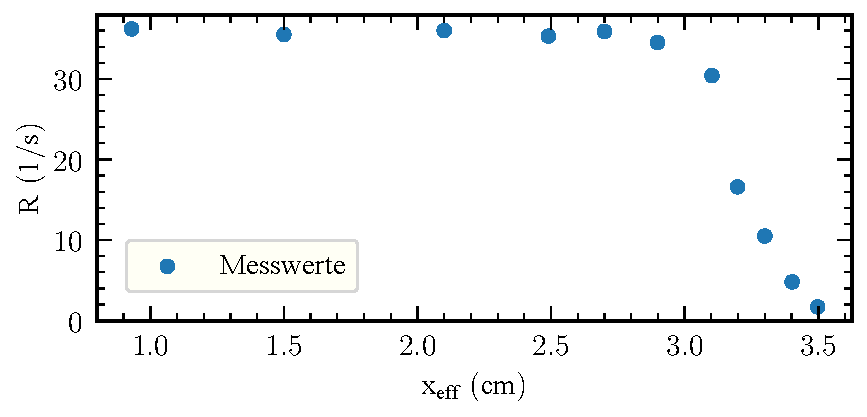
\includegraphics[width=\textwidth]{8_data}
		\end{minipage}
	\tcbline
		\begin{minipage}{\textwidth}
			\hspace{-1cm}
			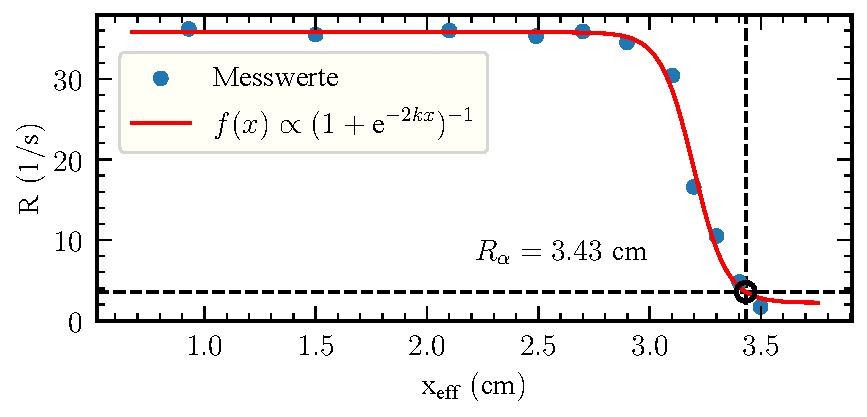
\includegraphics[width=\textwidth]{8_fit}
		\end{minipage}
		Fitfunktion als angepasste Heaviside Funktion \href{https://en.wikipedia.org/wiki/Heaviside_step_function}{[1]} scheint recht gut zu passen. 
		\( f(R_{\alpha}) \stackrel{!}{=} \tfrac{f_{\text{max}}}{10} \quad \Rightarrow \quad R_{\alpha} = 3.43 \unit{cm} \)
	\tcbline
		\begin{flalign*}
			R_{\alpha} &= 0.31 \left(\tfrac{E_{\text{kin}}}{1 \unit{MeV}}\right)^{3/2} \unit{cm} = 3.43 \unit{cm} &&\\[2ex]
			E_{\text{kin}} &= \dl{4.97 \unit{MeV}} &&
		\end{flalign*}
	\tcbline
		\begin{minipage}{\textwidth}
			\hspace{-1cm}
			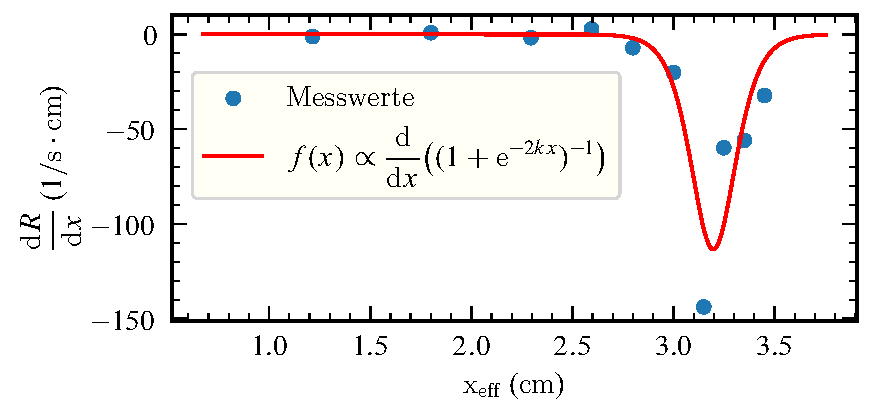
\includegraphics[width=\textwidth]{8_dd}
		\end{minipage}\\
	In blau numerisch differenzierte Werte $\big($über \( f'(x_n) = \tfrac{f(x_{n+1}) - f(x_n)}{x_{n+1} - x_n} \)$\big)$. In rot Ableitung der Fitfunktion aus c). Man erkennt sehr gut, dass bei ca. \( 3.2 \unit{cm} \) ein starker Fall ist, was physikalisch bedeutet, dass bei dieser Entfernung die \( \alpha- \)Teilchen ihre Energie deponieren. 
	\end{enumerate}
\end{mybox}

\begin{mybox}{Bethe-Bloch-Formel}
	\centering \(  \)
	\tcblower
		\begin{minipage}{\textwidth}
			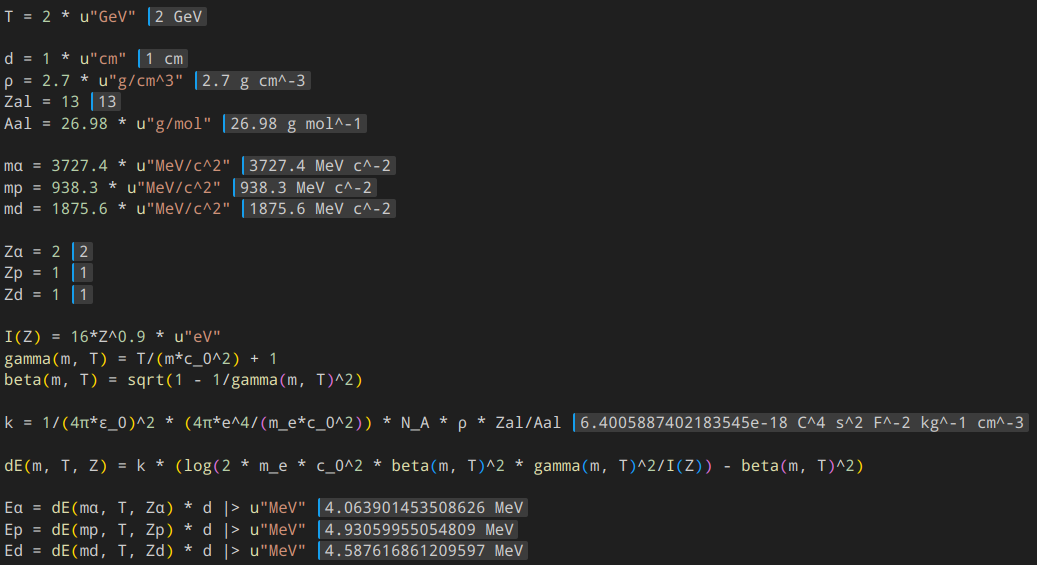
\includegraphics[width=\textwidth]{code}
		\end{minipage}
		\vspace{0.5cm} \\
		\( E_{\alpha} = 4.06 \unit{MeV};\quad E_p = 4.93 \unit{MeV};\quad E_d = 4.59 \unit{MeV} \)
	\tcbline
		\begin{minipage}{\textwidth}
			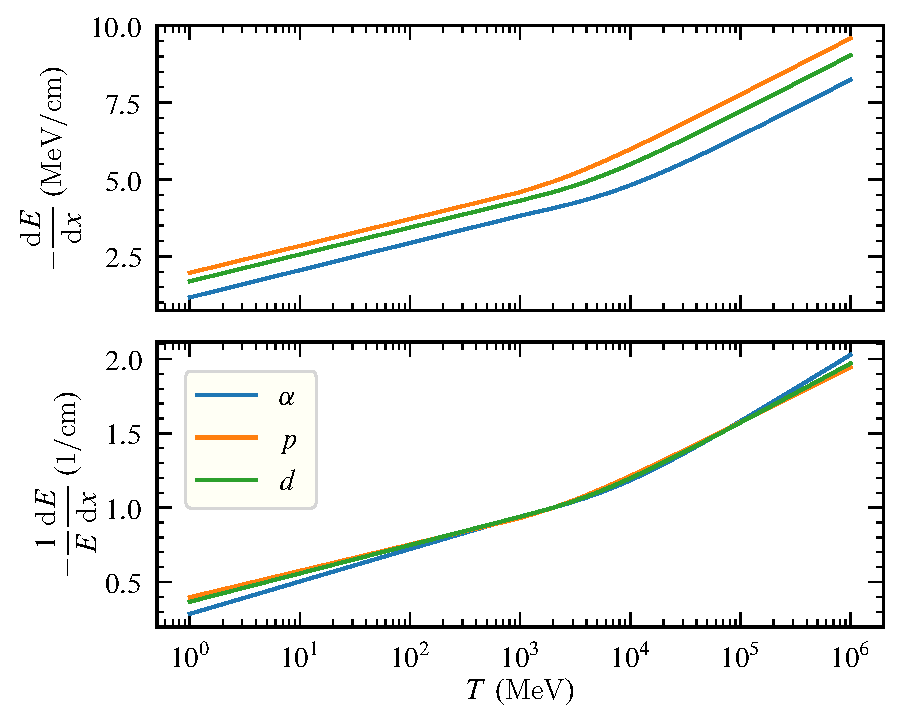
\includegraphics[width=\textwidth]{8_loglog}
		\end{minipage}
	\tcbline
		Nein, aufgrund der geringen Masse ist Bremsstrahlung bei Elektronen weitaus dominanter als Ionisierungsprozesse.
\end{mybox}

\begin{mybox}{Elektromagnetische Teilchenschauer}
	\centering \(  \)
	\tcblower
	\begin{enumerate}
		\item \(  \)
		\begin{tikzpicture}[scale=1.5]
			\matrix (m) [matrix of nodes, nodes in empty cells, row sep=0.5cm, column sep=1.5cm]
			{
%				m-1-1 & m-1-2 & m-1-3 & m-1-4 & m-1-5 \\
%				m-2-1 & m-2-2 & m-2-3 & m-2-4 & m-2-5 \\
%				m-3-1 & m-3-2 & m-3-3 & m-3-4 & m-3-5 \\
%				m-4-1 & m-4-2 & m-4-3 & m-4-4 & m-4-5 \\
%				m-5-1 & m-5-2 & m-5-3 & m-5-4 & m-5-5 \\
%				m-6-1 & m-6-2 & m-6-3 & m-6-4 & m-6-5 \\
%				m-7-1 & m-7-2 & m-7-3 & m-7-4 & m-7-5 \\
%				m-8-1 & m-8-2 & m-8-3 & m-8-4 & m-8-5 \\
				& & & & \\
				& & & & \\
				& & & & \\
				& & & & \\
				& & & & \\
				& & & & \\
				& & & & \\
				& & & & \\
			};
			
%			main particle
			\draw[thick, -Latex, green] 
			(m-3-1) edge (m-3-2) 
			(m-3-2) edge (m-3-3)
			(m-3-3) edge (m-3-4) 
			(m-3-4) edge (m-3-5);
%			photons
			\draw[thick, -Latex, snake arrow, blue] (m-3-2) -- (m-5-3);
			\draw[thick, -Latex, snake arrow, blue] (m-3-3) -- (m-2-4);
			\draw[thick, -Latex, snake arrow, blue] (m-3-4) -- (m-4-5);
			\draw[thick, -Latex, snake arrow, blue] (m-5-4) -- (m-6-5);
			\draw[thick, -Latex, snake arrow, blue] (m-7-4) -- (m-7-5);
%			secondary particle
			\draw[thick, -Latex, green] 
			(m-2-4) edge (m-2-5) 
			(m-5-3) edge (m-5-4) 
			(m-5-4) edge (m-5-5);
			\draw[thick, -Latex, red] 
			(m-2-4) edge (m-1-5)
			(m-5-3) edge (m-7-4) 
			(m-7-4) edge (m-8-5);
			
			\draw[Latex-Latex] (-1,-2) -- (0,-2) node [midway, above] {\( X_0 \)};
			
			\draw[thick, -Latex, green] (5,0) -- (6,0) node [pos=0, left] {\( e^- \)};
			\draw[thick, -Latex, red] (5,-0.5) -- (6,-0.5) node [pos=0, left] {\( e^+ \)};
			\draw[thick, -Latex, blue, snake arrow] (5,0.5) -- (6,0.5) node [pos=0, left] {\( \gamma \)};
		\end{tikzpicture}
	\tcbline
		\item \(  \)
		\begin{flalign*}
			E_{n \cdot X_0} &= \tfrac{E_0}{2^n} &&\\
			X_{\text{max}} &= \tfrac{\ln(\tfrac{E_0}{E_c})}{\ln(2)} X_0 &&\\[2ex]
			N_n &= N_{n-1} + 2N_{n-2} 
				= \dl{\tfrac{2}{3}2^n + \tfrac{1}{3}(-1)^n} &&
		\end{flalign*}
	\tcbline
		\item \( E_c = 84 \unit{MeV};\quad E_1 = 1 \unit{TeV};\quad E_2 = 10^8 \unit{TeV} \)
		\begin{flalign*}
			X_1 &= \frac{3}{2} \tfrac{\ln(\tfrac{E_1}{E_c})}{\ln(2)} X_0 
				= \dl{20.31 X_0} &&\\[2ex]
			X_2 &= \frac{3}{2} \tfrac{\ln(\tfrac{E_2}{E_c})}{\ln(2)} X_0 
				= \dl{60.17 X_0} &&\\	
		\end{flalign*}
	\tcbline
		\item \( H_0 = 8 \unit{km};\quad X_E = \unit{g/cm^2};\quad X_0 = 37.8 \unit{g/cm^2} \)
		\begin{flalign*}
			X_1 &\stackrel{!}{=} X_E \expo[-][h/H_0] &&\\
			\Rightarrow h &= -\ln(\tfrac{X_1}{X_E}) H_0 
				= \dl{2.35 \unit{km}} &&\\[2ex]
			X_2 &\stackrel{!}{=} X_E \expo[-][h/H_0] &&\\
			\Rightarrow h &= -\ln(\tfrac{X_2}{X_E}) H_0 
				= \dl{-6.34 \unit{km}} &&
		\end{flalign*}
	\tcbline
		\item \( h = 575 \unit{m} \)
		\begin{flalign*}
			X_{\text{max}} &= \tfrac{\ln(\tfrac{E_0}{E_c})}{\ln(2)} X_0 
				\stackrel{!}{=} X_E \expo[-][h/H_0] &&\\[2ex]
			E &= 2E_c \exp(2X_E/3X_0 \exp(-h/H_0))
				= \dl{10.32 \unit{TeV}} &&
		\end{flalign*}
	\end{enumerate}
\end{mybox}


\end{document}